\header{
    \headtitle{Le vieux curé de Paris} \label{le-vieux-cure-de-paris}
    %
    
    \insertComment{Sur l'air de "Chevalier de la table ronde".}{}
}

\enluminure{4}{\href{https://www.youtube.com/watch?v=B9DFAyLVnQ0}{J}}
$\left.\begin{tabular}{l}
\hspace{-0.4cm}
\textsc{e vais} vous raconter l'histoire
\\
\hspace{-0.4cm}
D'un vieux curé de Paris
\end{tabular}\right\rbrace$ bis
\\D'un vieux cu -- oui oui
\\D'un vieux cu -- la la
\\D'un vieux curé de Paris
\\
\bisdouble{Chaque fois qu'il dit sa messe}
{Son grand vicaire le suit}
\\Son grand vi -- oui oui
\\Son grand vi -- la la
\\Son grand vicaire le suit
\\
\bisdouble{Chaque fois qu'il monte en chaire}
{Tire un coupable d'enfer}
\\Tire un cou -- oui oui
\\Tire un cou -- la la
\\Tire un coupable d'enfer
\\
\bisdouble{Il aime une jeune bergère}
{Pour son troupeau de moutons}
\\Pour son trou -- oui oui
\\Pour son trou -- la la
\\Pour son troupeau de moutons
\\
\bisdouble{Il aime sa cuisinière}
{Pour ses festins d'Gargantua}
\\Pour ses fes -- oui oui
\\Pour ses fes -- la la
\\Pour ses festins d'Gargantua
\\
\bisdouble{Il possède une rivière}
{Au bord d'elle il se complaît}
\\Au bord d'elle -- oui oui
\\Au bord d'elle -- la la
\\Au bord d'elle il se complaît
\breakpage
Il aime la botanique
\\Il en cultive les fleurs
\\Il en cul -- oui oui
\\Il en cul -- la la
\\Il en cultive les fleurs
\\\\Le héros de cette histoire
\\Est Pinaud, curé de Paris
\\Pinaud cu -- oui oui
\\Pinaud cu -- la la
\\Pinaud curé de Paris
\\
\begin{center}
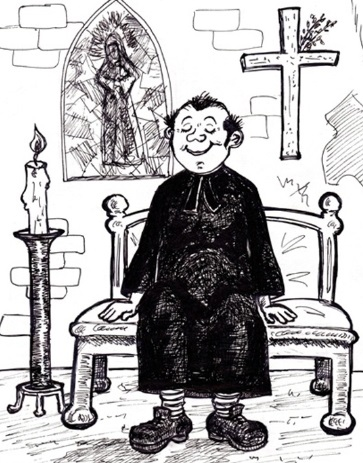
\includegraphics[width=0.8\textwidth]{images/cure_paris.jpg}
\end{center}

\breakpage